\documentclass[10pt]{article}
\usepackage[margin=0.85in]{geometry}
\usepackage{graphicx}
\usepackage{booktabs}
\usepackage{amsmath,amssymb}
\usepackage{hyperref}
\usepackage{xcolor}
\usepackage{caption}
\usepackage{subcaption}
\usepackage{microtype}
\usepackage[section]{placeins}
\captionsetup{font=small,labelfont=bf}
\hypersetup{colorlinks=true,linkcolor=blue!60!black,urlcolor=blue!60!black,citecolor=blue!60!black}
\graphicspath{{figures/}}
\setlength{\parskip}{3pt}
\newcommand{\lr}{\eta}
\newcommand{\budgethours}{24 GPU hours (22.2 hours of logged training plus stopped runs and one retry)}
\newcommand{\studentfailures}{\item My runs: d8-ema01 collapsed to 6.875 at 0.00075, 0.003 and 0.006; d8-block2 at 0.018 trained to 3.600 (rate too high, no NaN); gru-dual went non-finite at step 1866 (0.003) and step 827 (0.0015); gru-linear went non-finite at step 1960 (0.003); these three were stopped by hand.
\item Infrastructure: Modal reused one container for consecutive jobs, so after a few jobs torch.compile hit its recompile limit and the job crashed before its first step, and the next job in that container logged into the crashed job's W\&B run (the W\&B run named d8-attention at 0.003 contains the d8-block4 at 0.003 training). I set the training function to one job per container, relaunched the five affected runs, and recomputed every reported loss from the saved checkpoints in FP32 instead of trusting W\&B names.}

\newcommand{\ablationparagraph}{\paragraph{Ablations.} All three ablations ran at $\lr=0.003$, where the full GRU reaches 3.188. Removing the reset gate costs 0.10 nats (3.285): the candidate then always reads the whole state and cannot write a fresh value into a unit while keeping the old one around for the update gate's decision. Computing both gates from the input alone costs 0.05 (3.235): the model still has a reset and an update gate, but it can no longer decide to forget based on what it currently holds. Dropping the candidate tanh is fatal: the gated linear map produced non-finite losses at step 1960 and the run was stopped, because without the squashing nonlinearity the candidate scale is set by $W x + U(r\odot h)$ and the recurrence has no bounded fixed point. The no-reset cell also saturates like the tanh cell (80\% of its last layer units beyond 0.95, hidden RMS 0.9, Figure~\ref{fig:p4time}) and freezes its upper layers in time (cosine 0.995 between $h_t$ and $h_{t-64}$ in layers 3 and 4, against 0.64 to 0.84 for the GRU), so without the reset the model falls back to the tanh RNN's strategy of a static upper state. Both the GRU and these ablations stay well ahead of the tanh baseline (3.516): the single biggest gain in P4 comes from the convex, gated update itself, the reset and the recurrent terms in the gates are second order, and a saturating candidate is necessary.}
\newcommand{\comparisonresults}{(pending)}

\title{CS312 Assignment 4: Transformers vs RNNs}
\author{Aidan White (whitedeer)}
\date{October 2026}

\begin{document}
\maketitle

\section{Setup}

All models share one recipe from the course codebase: vocabulary 4096, context 1024, width 512, batch 64 sequences, 600{,}000 training sequences (614.4M tokens, 9{,}374 steps), AdamW with weight decay 0.1, 1\% linear warmup followed by linear decay to zero, gradient clipping at norm 1, mixed precision training, model seed 42 and data seed 42. The metric throughout is the validation loss on the held out DCLM split after the last step (lower is better). Peak learning rate is the only hyperparameter swept. P1 and P2 use the 105 supplied reference runs (21 variants, five rates each, centred on the instructor's trial rate). P3 and P4 runs were trained for this report on H100s in my Modal environment with the same recipe and are listed with their rates in each section.

\paragraph{Diagnostics.} Checkpoint probes run the FP32 copy of each model on the same eight held out validation sequences (full backpropagation through time for the RNNs). For every branch input along the depth stream and for the final stream before the output norm I record the activation RMS, the gradient RMS of the full next token loss and of the loss on the final token only, the RMS ratio of the raw branch output to its input, and the cosine between consecutive stream states. For attention layers I record, for 32 query positions, the softmax mass on the first token, the mass on the query itself and the mean attention lag, which I compare with a uniform causal prefix baseline (mass $1/(t+1)$ on each of the $t+1$ visible keys, mean lag $t/2$). For recurrent layers I record per time step the hidden state RMS, the hidden state gradient RMS under both losses, the fraction of $|h|>0.95$ and the cosine between $h_t$ and $h_{t-\ell}$ for lags 1, 4, 16, 64. Context tests rerun the final token prediction with only the $k$ most recent input tokens (original positions preserved, recurrent state reset), with and without the first token restored, on 64 validation sequences. Three checkpoints are probed per selected run: the seed 42 initialisation, step 100 and the final model. All probe code is in \texttt{experiments/a4\_stability/measure\_all.py} and the plotting code in \texttt{report/plot\_*.py}; the figures only use these probe files and the W\&B logs.

\paragraph{Compute.} Training used about \budgethours{} of the 48 GPU hour budget. The reference P1/P2 probes ran on CPU containers because both GPU slots were busy with P3/P4 training; results are identical in FP32 up to accumulation order.

\section{P1: Transformer depth}

\subsection{Learning rate sweeps}
Figure~\ref{fig:p1lr} and Table~\ref{tab:p1} summarise the 50 supplied transformer runs. The baseline d8 reaches 2.927 at $\lr=0.003$ and is flat within 0.02 over a factor of four in rate. Removing residual connections is fatal at every rate: all five runs sit at 6.875, the unigram level, so the model never learns to use its input. Removing pre-normalisation and post-norm both shift the usable rates down by a factor of three and lose 0.14 to 0.22 nats at their best rate; no-prenorm produces non-finite gradients at $\lr\geq 0.002$ and post-norm collapses at $0.004$. Removing QK normalisation costs little at the centre rate (2.951) but the loss explodes to 3.83 and 4.20 at $2\times$ and $4\times$ the centre: QK norm buys learning rate headroom rather than loss. Removing RoPE costs 0.14 nats at every rate, and removing the final norm costs 0.03 at the centre but degrades at high rates. The three gates all help a little: gated residuals 2.910, gated attention 2.917 and gated norm 2.939 (at its own centre of 0.00225, where the sweep is flat from 0.00225 to 0.009).

\begin{figure}[h]\centering
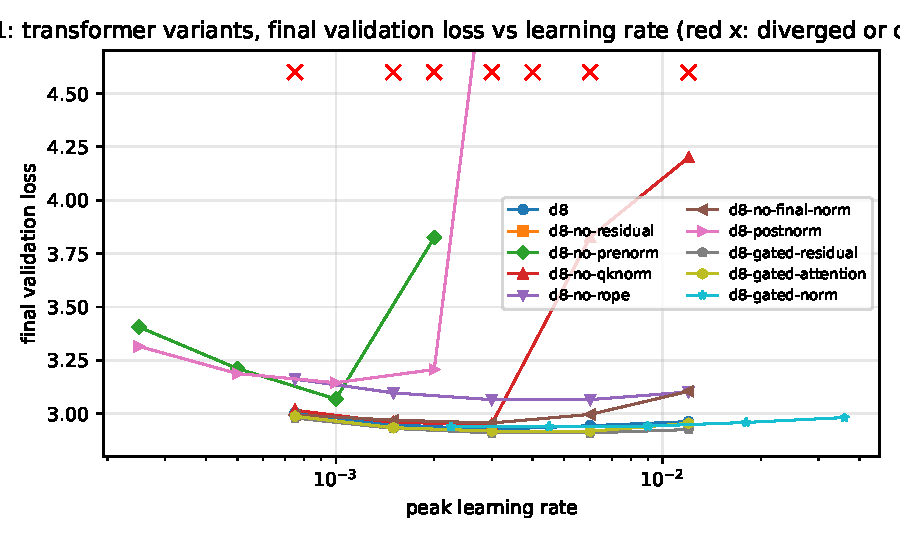
\includegraphics[width=.72\linewidth]{p1_lr_sweep.pdf}
\caption{P1 learning rate sweeps. Red crosses mark runs with non-finite gradients or final loss above 4.6 (no-residual at every rate sits at 6.875, off the axis).}
\label{fig:p1lr}
\end{figure}

\begin{table}[h]\centering\small
\caption{P1 final validation loss per rate (columns are $0.25\times$ to $4\times$ each variant's centre; best in bold; div. means non-finite). Params in millions.}
\label{tab:p1}
\begin{tabular}{lrrrrrrr}\toprule
variant & best $\lr$ & $0.25\times$ & $0.5\times$ & $1\times$ & $2\times$ & $4\times$ & params (M)\\\midrule
d8 & 0.003 & 3.004 & 2.948 & \textbf{2.927} & 2.943 & 2.963 & 34.6 \\
d8-no-residual & 0.00075 & \textbf{6.875} & 6.875 & 6.875 & 6.875 & 6.875 & 34.6 \\
d8-no-prenorm & 0.001 & 3.406 & 3.211 & \textbf{3.069} & 3.825 & div. & 34.6 \\
d8-no-qknorm & 0.003 & 3.016 & 2.959 & \textbf{2.951} & 3.827 & 4.200 & 34.6 \\
d8-no-rope & 0.003 & 3.162 & 3.097 & \textbf{3.065} & 3.066 & 3.101 & 34.6 \\
d8-no-final-norm & 0.003 & 2.994 & 2.969 & \textbf{2.956} & 2.996 & 3.104 & 34.6 \\
d8-postnorm & 0.001 & 3.315 & 3.188 & \textbf{3.145} & 3.207 & 6.875 & 34.6 \\
d8-gated-residual & 0.003 & 2.980 & 2.931 & \textbf{2.910} & 2.910 & 2.925 & 38.8 \\
d8-gated-attention & 0.006 & 2.987 & 2.934 & 2.918 & \textbf{2.917} & 2.955 & 34.6 \\
d8-gated-norm & 0.00225 & \textbf{2.939} & 2.940 & 2.941 & 2.959 & 2.982 & 38.8 \\
\bottomrule\end{tabular}

\end{table}

\subsection{Activation and gradient RMS across depth}
Figure~\ref{fig:p1depth} shows the FP32 probes of the final checkpoints at each variant's best rate, and Figure~\ref{fig:p1stages} tracks the baseline from initialisation to the end. In the baseline the residual stream RMS grows monotonically from 0.15 at the embedding to 24 before the final norm, with most of the growth in the first two blocks; the raw branch outputs are 6 to 20 times larger than their input at the first attention branch and then settle at 0.3 to 0.5 of the stream, so each later block is a small correction to a large stream. The gradient of the full loss with respect to the stream decays only from $1.4\times10^{-5}$ at the embedding to $3\times10^{-7}$ at the top and is nearly flat over the middle twelve branches, as the additive path guarantees; the last-token gradient is about 50 times larger (it is not averaged over 1023 targets) and has the same shape. The cosine between consecutive stream states is above 0.9 from block 2 onward: the stream changes direction mostly at the bottom. Training compresses the gradient range at the bottom (the embedding gradient falls by 1000 between init and step 100 while the top stays put), consistent with the first blocks growing the stream quickly.

The no-residual model is the opposite picture: at the final checkpoint the stream RMS grows from $2\times10^{-3}$ to 430 across 16 branches, the cosine between consecutive states is 0, and the gradient RMS spans $10^{-20}$ to $10^{-9}$ from bottom to top, so the lower half of the network is dead and the top learns a unigram predictor. The no-prenorm and post-norm models keep the stream between 0.05 and 1 but pay for it with gradients that are 10 to 100 times larger than the baseline's at every depth, which is why their rates had to be lowered. The no-final-norm model learns to keep its top stream at 1.4 instead of 24, because the head sees the raw stream. Gated residuals have the largest branch to input ratio (1.9 on average), meaning the gate lets the branches write more.

\begin{figure}[h]\centering
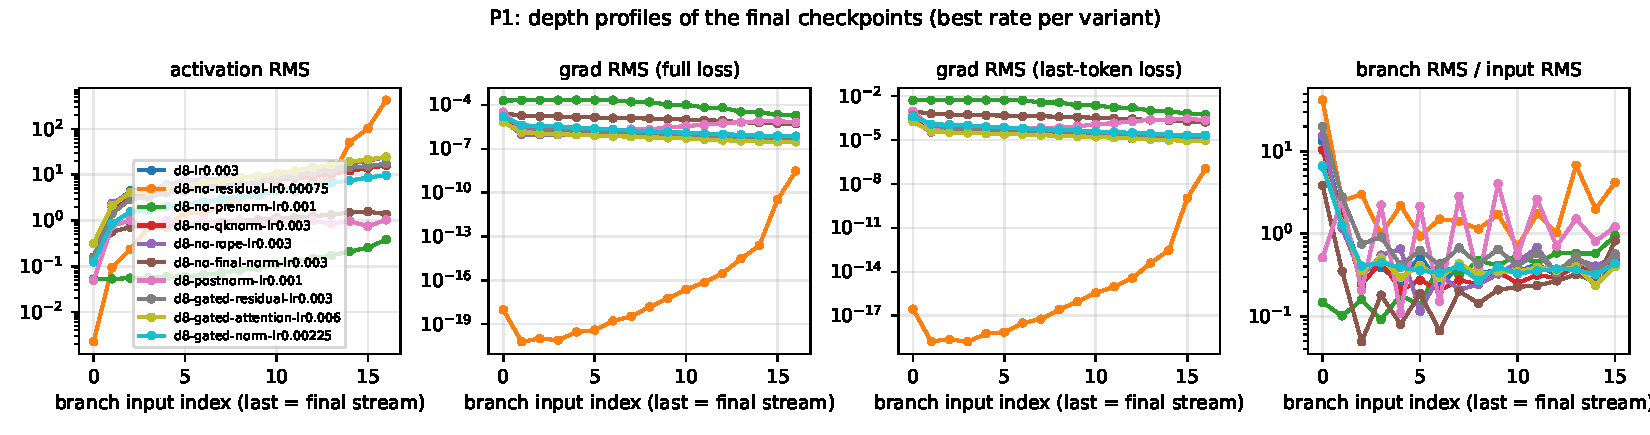
\includegraphics[width=\linewidth]{p1_depth_final.pdf}
\caption{P1 depth profiles of the final checkpoints. Index 0 is the embedding entering the first attention branch, odd indices are MLP branch inputs, index 16 is the final stream before the output norm.}
\label{fig:p1depth}
\end{figure}

\begin{figure}[h]\centering
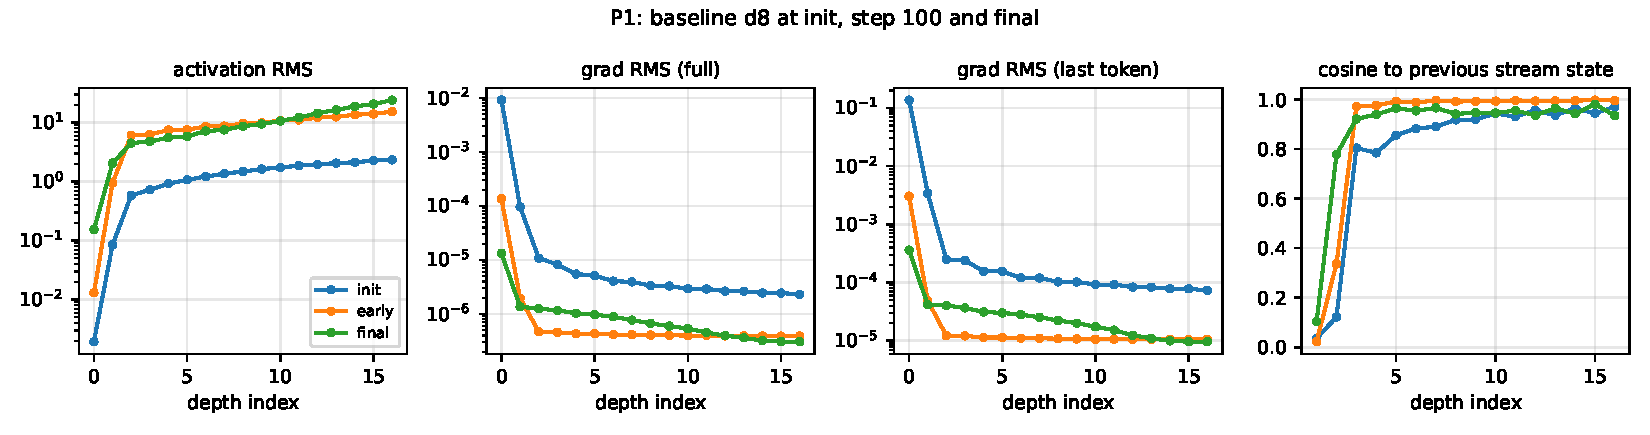
\includegraphics[width=\linewidth]{p1_d8_stages.pdf}
\caption{Baseline d8 at initialisation, step 100 and the final checkpoint.}
\label{fig:p1stages}
\end{figure}

\subsection{Attention patterns and sinks}
Figure~\ref{fig:p1attn} compares attention mass on the first token, mass on the query itself and mean lag with the uniform causal prefix baseline. Every trained model with residuals puts far more mass on the first token than uniform attention would: at position 1000 the baseline averages 0.08 on the first token (100 times uniform) and the no-prenorm and no-final-norm models 0.3 to 0.4. This is the attention sink. The mass on self flattens at 0.03 to 0.1 rather than decaying as $1/(t+1)$, and the mean lag is close to but below the uniform $t/2$, so the layers are a mixture of near uniform averaging heads, sink dominated heads and local heads. The no-residual model matches the uniform baseline exactly in all three statistics: its attention never learned anything. The two gated variants and the plain baseline have the smallest sinks (gated attention falls to 0.01 at the end of the context), consistent with the gate doing the job of switching heads off that the sink otherwise does. Without RoPE the sink is as strong as the baseline's but the model is 0.14 nats worse and its context test below shows that it depends on the first token to work at all.

\begin{figure}[h]\centering
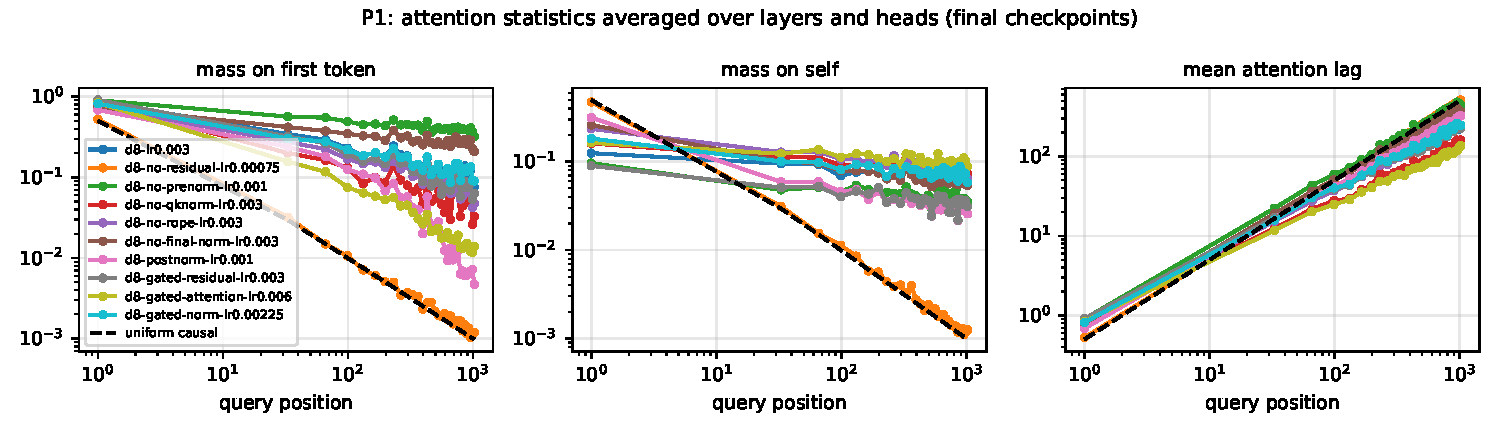
\includegraphics[width=\linewidth]{p1_attention.pdf}
\caption{P1 attention statistics on 32 query positions, averaged over heads and layers of the final checkpoints. Dashed: uniform causal prefix.}
\label{fig:p1attn}
\end{figure}

\subsection{Context use}
Figure~\ref{fig:p1ctx} reruns the last token prediction with only the $k$ most recent input tokens. The baseline loses 6.5 nats with one token of context, 1.7 with 16, 0.4 with 64 and under 0.1 with 256 or more, so the model relies on about 100 tokens for most of its loss but still gains measurably from the full window. Restoring the first token (a sink for every head) halves the penalty at short contexts. The no-RoPE model is the pathological case: without the first token its loss increase is 4.5 nats even with 512 recent tokens, and with the first token restored it is the model that recovers fastest. Its heads have no positional signal, so they use the first token as a fixed anchor and fail without it.

\begin{figure}[h]\centering
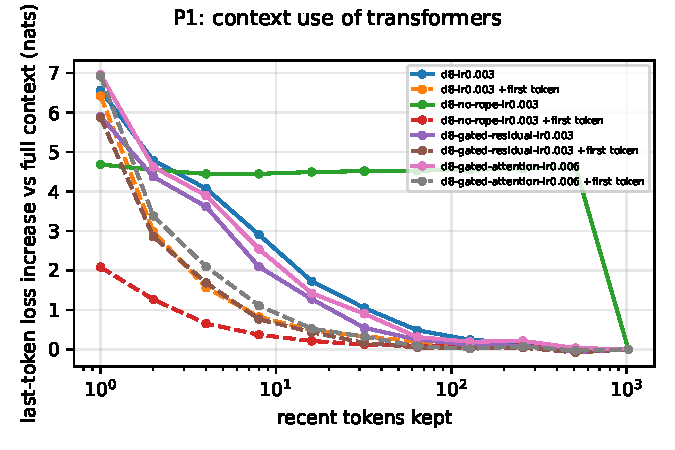
\includegraphics[width=.5\linewidth]{p1_context.pdf}
\caption{P1 context tests: increase of the last token loss over the full window loss, 64 validation sequences. Dashed lines restore the first token.}
\label{fig:p1ctx}
\end{figure}

\section{P2: RNN depth and time}

\subsection{Learning rate sweeps}
Figure~\ref{fig:p2lr} and Table~\ref{tab:p2} cover the 55 supplied RNN runs. The 1-layer plain tanh RNN reaches 4.033 at $\lr=0.003$; stacking four plain layers does not help (4.081 at $0.001$) and collapses to the unigram loss 6.875 at $0.002$ and $0.004$. The modern 4-layer RNN (pre-norm, depth residuals, SwiGLU MLPs) reaches 3.516 at $\lr=0.002$, half a nat better than either plain model, and is the only RNN family that is stable across the whole sweep. Among its ablations the differences are small at the best rate: gated residuals 3.496, gated norm 3.506, post-norm 3.512, gated output 3.513, final norm 3.521, no pre-norm 3.482 (its best, at $0.002$), no residual 3.581, RoPE on the recurrent input 3.566. The differences show up at higher rates: no pre-norm has non-finite gradients at $0.004$, post-norm climbs to 4.26 and 6.39 at $0.002$ and $0.004$ with its global activation RMS reaching 4000 (Figure~\ref{fig:p2rms}), and final norm, gated residual and gated output lose 0.1 to 0.15 nats at $2\times$ the centre. Pre-norm and depth residuals buy stability and rate headroom more than loss at the best rate, which matches P1.

\begin{figure}[h]\centering
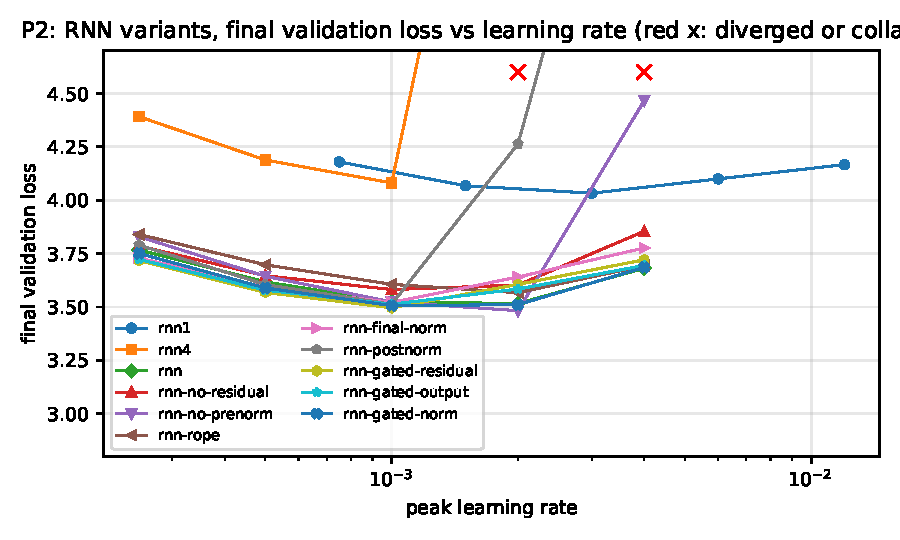
\includegraphics[width=.72\linewidth]{p2_lr_sweep.pdf}
\caption{P2 learning rate sweeps. Red crosses mark non-finite or collapsed runs.}
\label{fig:p2lr}
\end{figure}

\begin{table}[h]\centering\small
\caption{P2 final validation loss per rate (columns $0.25\times$ to $4\times$ each variant's centre; best in bold).}
\label{tab:p2}
\begin{tabular}{lrrrrrrr}\toprule
variant & best $\lr$ & $0.25\times$ & $0.5\times$ & $1\times$ & $2\times$ & $4\times$ & params (M)\\\midrule
rnn1 & 0.003 & 4.179 & 4.068 & \textbf{4.033} & 4.100 & 4.167 & 4.7 \\
rnn4 & 0.001 & 4.391 & 4.188 & \textbf{4.081} & 6.875 & 6.875 & 6.3 \\
rnn & 0.002 & 3.767 & 3.617 & 3.523 & \textbf{3.516} & 3.681 & 17.3 \\
rnn-no-residual & 0.001 & 3.785 & 3.646 & \textbf{3.581} & 3.602 & 3.855 & 17.3 \\
rnn-no-prenorm & 0.002 & 3.829 & 3.644 & 3.523 & \textbf{3.482} & 4.467 & 17.3 \\
rnn-rope & 0.002 & 3.839 & 3.697 & 3.606 & \textbf{3.566} & 3.694 & 17.3 \\
rnn-final-norm & 0.001 & 3.729 & 3.592 & \textbf{3.521} & 3.640 & 3.776 & 17.3 \\
rnn-postnorm & 0.001 & 3.789 & 3.605 & \textbf{3.512} & 4.263 & 6.389 & 17.3 \\
rnn-gated-residual & 0.001 & 3.717 & 3.568 & \textbf{3.496} & 3.605 & 3.721 & 19.4 \\
rnn-gated-output & 0.001 & 3.722 & 3.578 & \textbf{3.513} & 3.584 & 3.694 & 17.3 \\
rnn-gated-norm & 0.001 & 3.751 & 3.589 & \textbf{3.506} & 3.511 & 3.685 & 19.4 \\
\bottomrule\end{tabular}

\end{table}

\begin{figure}[h]\centering
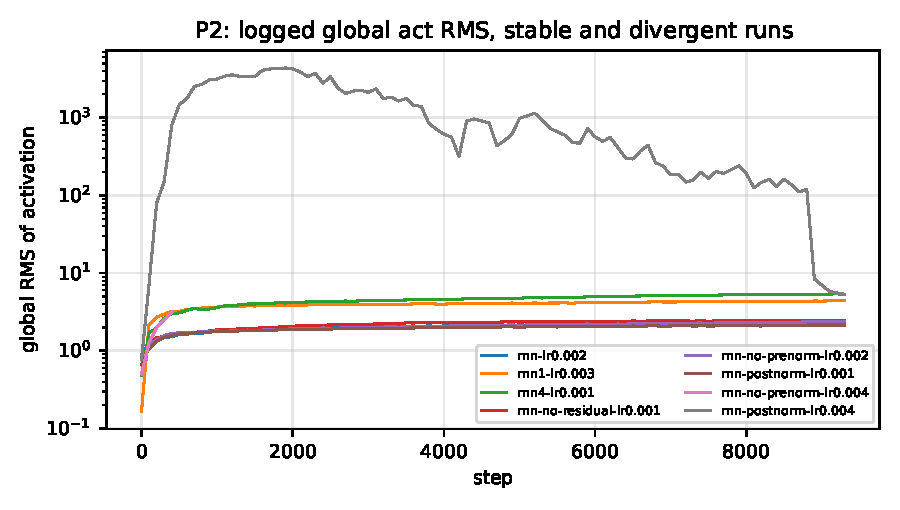
\includegraphics[width=.49\linewidth]{p2_rms_act.pdf}
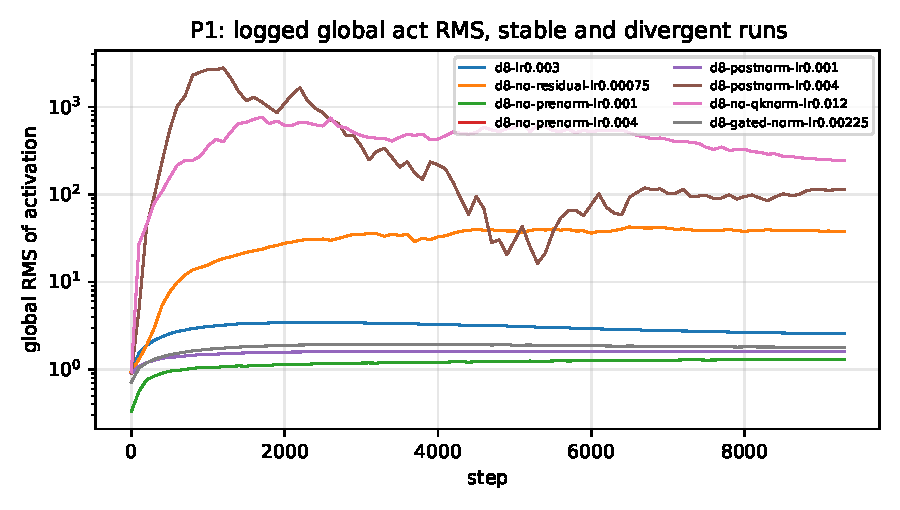
\includegraphics[width=.49\linewidth]{p1_rms_act.pdf}
\caption{Logged global activation RMS during training for stable and unstable RNN (left) and transformer (right) runs.}
\label{fig:p2rms}
\end{figure}

\subsection{Hidden state gradients, RMS and saturation}
Figure~\ref{fig:p2time} shows the last recurrent layer of the three main models on the final checkpoints. All three keep the hidden state RMS between 0.78 and 0.9, and 35\% (1 layer) to 55\% (4 layers) of the tanh units are saturated beyond 0.95 at every step. Under the full loss the gradient reaching $h_t$ is flat over time, because every position has its own target. Under the last-token loss the picture is the classic one: the gradient falls by about 32 orders of magnitude across the 1024 steps for the 1-layer RNN, and the plain 4-layer and modern RNNs underflow to zero after 250 and 90 steps respectively. The modern RNN has the shortest temporal gradient reach of the three because its upper layers are smooth in time (cosine between $h_t$ and $h_{t-64}$ is 0.93 in layer 4 versus 0.15 in the 1-layer model, Figure~\ref{fig:p2layers}): information flows forward along the depth residual, not back along time. The plain 4-layer model has intermediate smoothness (0.12 in layer 1 to 0.48 in layer 4) and shows the depth problem instead: its layer 1 hidden state gradient under the full loss is 3 times smaller than its layer 4 gradient at init and the stream gradient drops by 10 across the stack (Figure~\ref{fig:p2depth}).

\begin{figure}[h]\centering
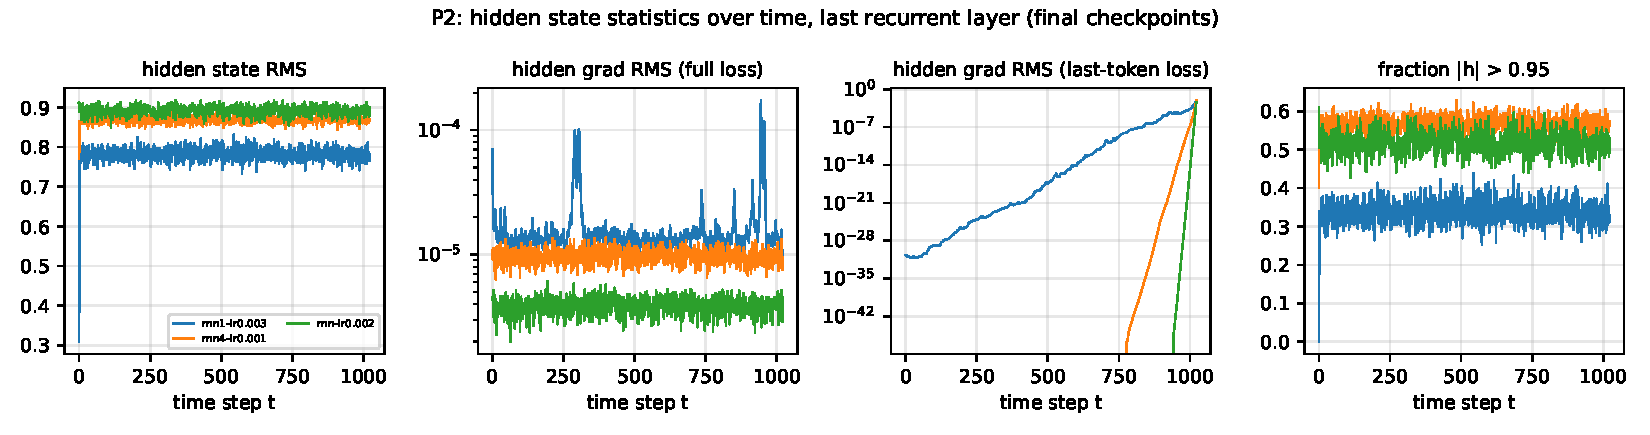
\includegraphics[width=\linewidth]{p2_temporal_plain_vs_modern.pdf}
\caption{Last recurrent layer over time for the 1-layer, plain 4-layer and modern RNNs (final checkpoints, 8 sequences).}
\label{fig:p2time}
\end{figure}

\begin{figure}[h]\centering
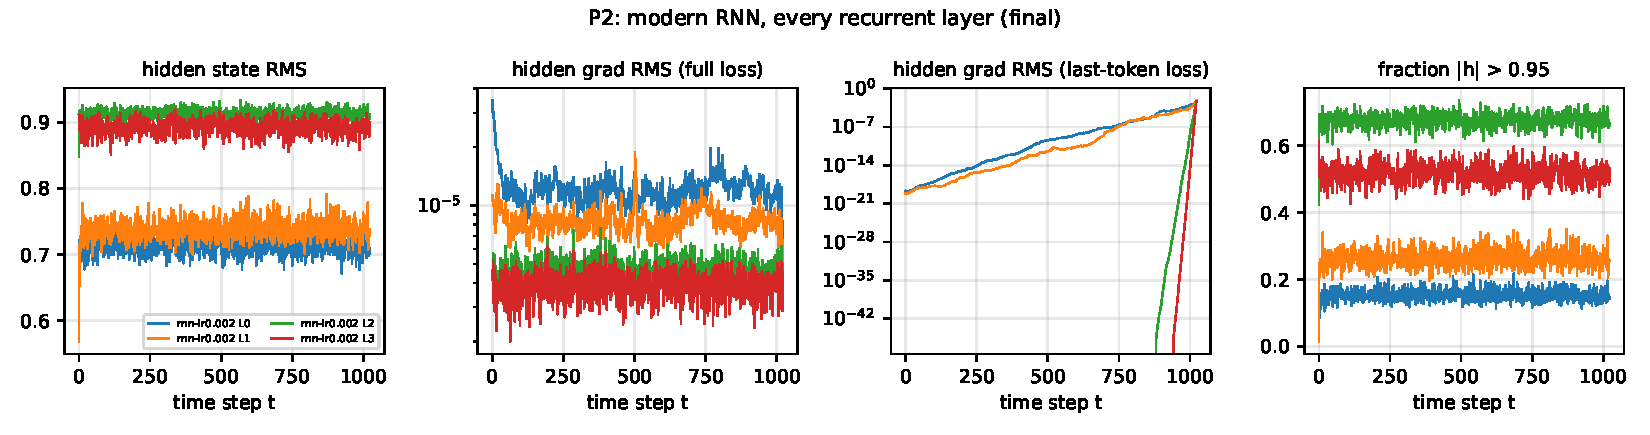
\includegraphics[width=\linewidth]{p2_temporal_rnn_layers.pdf}
\caption{Modern RNN: every recurrent layer over time (final checkpoint). Lower layers change fast, upper layers hold an almost constant state.}
\label{fig:p2layers}
\end{figure}

\subsection{Depth}
Figure~\ref{fig:p2depth} gives the depth profiles. The modern RNN's stream grows from 0.11 to 1.7 over 8 branches, with the cosine between consecutive stream states between 0.75 and 0.97, so, as in the transformer, each branch is a correction to a shared stream. Without depth residuals the stream has cosine 0 between consecutive states and the branch to input ratio alternates between 0.3 and 5: the recurrent branches contract and the MLPs expand. The no-residual, no-prenorm and post-norm ablations also have the largest upper layer temporal cosines (0.998 and 0.999 in layers 3 and 4 for no-prenorm and RoPE), that is, their upper layers have essentially frozen their hidden state and act as feedforward layers. Figure~\ref{fig:p2stages} shows that, unlike the transformer, the modern RNN's depth profile is already in its final shape at initialisation; training changes the embedding gradient by 10 and little else.

\begin{figure}[h]\centering
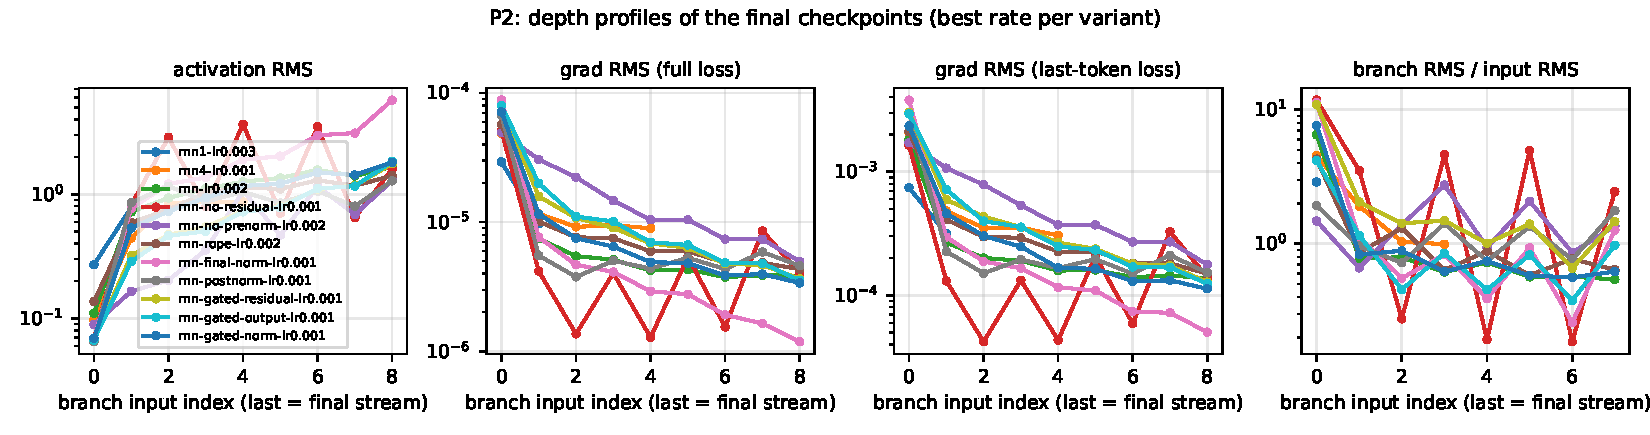
\includegraphics[width=\linewidth]{p2_depth_final.pdf}
\caption{P2 depth profiles (final checkpoints, best rate per variant). Even indices are recurrent branch inputs, odd are MLP inputs, index 8 is the final stream.}
\label{fig:p2depth}
\end{figure}

\begin{figure}[h]\centering
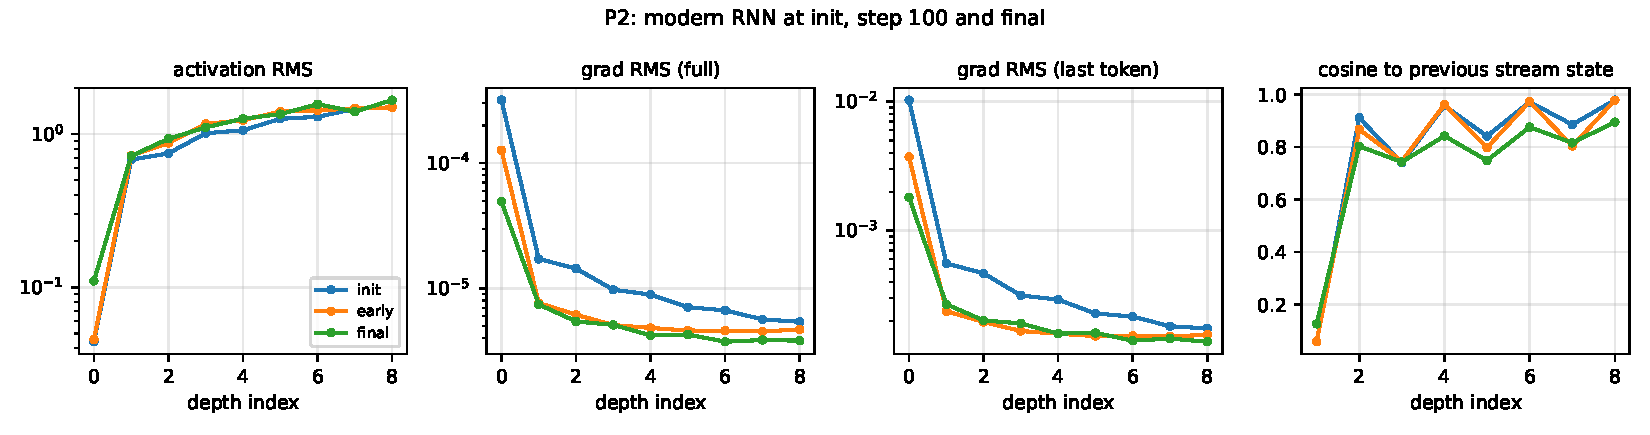
\includegraphics[width=\linewidth]{p2_rnn_stages.pdf}
\caption{Modern RNN at initialisation, step 100 and the final checkpoint.}
\label{fig:p2stages}
\end{figure}

\subsection{Context use and the first token}
Table~\ref{tab:p2ctx} gives the RNN context tests. With the first token restored all RNNs lose about 1.2 to 1.9 nats with one recent token, 0.2 to 0.5 with four and nothing measurable beyond 64, in line with the gradient reach above. Without the first token the plain RNNs are unaffected beyond 16 tokens, but the modern RNN loses 40 to 56 nats at every context length, including 512 tokens. Its upper layers hold a near constant state, that state is set by the first token (which the model always sees at position 0 in training), and starting the recurrence from $h_0$ on a mid-document token drives it into a regime from which it never recovers. The RoPE variant behaves the same way, with a 700 nat increase at one token. This is the recurrent analogue of the no-RoPE transformer's dependence on the sink token, and it is why the handout asks for the first token to be restored and the state to be reset correctly.

\begin{table}[h]\centering\small
\caption{Increase of the last token loss (nats) when only $k$ recent tokens are kept; recurrent state reset; final checkpoints; 64 sequences.}
\label{tab:p2ctx}
\begin{tabular}{llrrrrrr}\toprule
model & first token & $k=1$ & 2 & 4 & 16 & 64 & 512\\\midrule
rnn1 & dropped & 1.57 & 0.74 & 0.23 & 0.01 & 0.01 & 0.00\\
rnn1 & restored & 1.22 & 0.67 & 0.28 & 0.03 & 0.00 & 0.00\\
rnn4 & dropped & 3.48 & 2.75 & 1.06 & 0.04 & 0.01 & 0.00\\
rnn4 & restored & 1.27 & 0.61 & 0.26 & 0.04 & 0.00 & 0.00\\
rnn (modern) & dropped & 42.3 & 50.5 & 54.9 & 56.1 & 49.1 & 54.6\\
rnn (modern) & restored & 1.91 & 1.07 & 0.50 & 0.16 & 0.00 & 0.00\\
rnn-gated-residual & dropped & 2.27 & 1.07 & 0.43 & 0.11 & 0.00 & 0.00\\
rnn-gated-residual & restored & 1.86 & 1.03 & 0.44 & 0.15 & 0.03 & 0.00\\
d8 transformer & dropped & 6.56 & 4.78 & 4.07 & 1.73 & 0.48 & 0.00\\
d8 transformer & restored & 6.42 & 2.98 & 1.56 & 0.47 & 0.19 & 0.00\\
d8 no RoPE & dropped & 4.68 & 4.55 & 4.44 & 4.49 & 4.52 & 4.61\\
d8 no RoPE & restored & 2.08 & 1.26 & 0.65 & 0.21 & 0.09 & 0.00\\
\bottomrule\end{tabular}
\end{table}

\section{P3: Attention residuals}
\paragraph{My own scheme: gated attention reads on top of the additive stream.}
The supplied variants replace the additive residual, and the ones that route (uniform, attention, blocked attention) must learn where each branch reads from. My variant keeps the additive stream and adds the routed read as a correction that starts switched off:
\[
x_{j+1} = x_j + F_j\!\left(x_j + g_j\,\mathrm{Attn}_j(x_0, u_1, \dots, u_j)\right), \qquad y = x_L + g_L\,\mathrm{Attn}_L(x_0, u_1, \dots, u_L),
\]
where $u_j = F_j(\cdot)$ are the raw branch outputs, $\mathrm{Attn}_j$ is the same normalized key, learned query mixer as the full attention residual variant and $g_j$ are scalar gates initialised at zero. At initialisation this model is bit for bit the baseline, so it inherits the baseline's signal propagation and its learning rate; the routers only matter once $g_j$ moves away from zero, and the gradient of $g_j$ is the inner product of the routed read with the branch input gradient, so a gate only opens when the routed read helps. Class \texttt{GatedRouteDepth} in \texttt{p3\_attention\_residuals.py}; variants \texttt{d8-route} and \texttt{rnn-route}.

\subsection{Runs and losses}
Tables~\ref{tab:p3t} and~\ref{tab:p3r} list every P3 run (FP32 validation loss recomputed on the saved checkpoint over the full 1000 sequence validation set; these agree with the logged bf16 values to three decimals). Transformer variants were run at $\lr\in\{0.003, 0.006\}$ (block 2 at its own centre, $\{0.0045, 0.009\}$), RNN variants at $\{0.001, 0.002\}$, and the range was extended once where the best rate sat on the edge (block 2 to 0.018, EMA 0.1 down to 0.00075).

\begin{table}[h]\centering\small
\caption{P3 transformers (d8). Best rate per variant in bold.}
\label{tab:p3t}
\begin{tabular}{lp{0.78\linewidth}}\toprule
variant & final validation loss per peak rate\\\midrule
d8 (supplied) & $\lr$=0.003: 2.927 (best of five) \\
d8-half & $\lr$=0.003: \textbf{2.933}; $\lr$=0.006: 2.938 \\
d8-ema01 & $\lr$=0.00075: \textbf{6.875}; $\lr$=0.003: 6.875; $\lr$=0.006: 6.875 \\
d8-ema09 & $\lr$=0.003: \textbf{2.950}; $\lr$=0.006: 2.969 \\
d8-uniform & $\lr$=0.003: \textbf{2.924}; $\lr$=0.006: 2.939 \\
d8-attention & $\lr$=0.003: \textbf{2.904}; $\lr$=0.006: 2.916 \\
d8-block2 & $\lr$=0.0045: 2.917; $\lr$=0.009: \textbf{2.900}; $\lr$=0.018: 3.600 \\
d8-block4 & $\lr$=0.003: 2.916; $\lr$=0.006: \textbf{2.910} \\
d8-route & $\lr$=0.003: \textbf{2.915}; $\lr$=0.006: 2.927 \\
\bottomrule\end{tabular}

\end{table}
\begin{table}[h]\centering\small
\caption{P3 modern RNNs.}
\label{tab:p3r}
\begin{tabular}{lp{0.78\linewidth}}\toprule
variant & final validation loss per peak rate\\\midrule
rnn (supplied) & $\lr$=0.002: 3.516 (best of five) \\
rnn-half & $\lr$=0.001: \textbf{3.503}; $\lr$=0.002: 3.538 \\
rnn-ema01 & $\lr$=0.001: \textbf{3.572}; $\lr$=0.002: 3.589 \\
rnn-ema09 & $\lr$=0.001: \textbf{3.505}; $\lr$=0.002: 3.512 \\
rnn-uniform & $\lr$=0.001: \textbf{3.572}; $\lr$=0.002: 3.583 \\
rnn-attention & $\lr$=0.001: 3.550; $\lr$=0.002: \textbf{3.547} \\
rnn-block2 & $\lr$=0.001: \textbf{3.535}; $\lr$=0.002: 3.577 \\
rnn-block4 & $\lr$=0.001: \textbf{3.515}; $\lr$=0.002: 3.578 \\
rnn-route & $\lr$=0.001: \textbf{3.518}; $\lr$=0.002: 3.522 \\
\bottomrule\end{tabular}

\end{table}

\paragraph{Transformer.} Replacing the additive skip is mostly a loss. EMA with $\beta=0.1$ collapses to the unigram loss 6.875 at all three rates: with $x' = 0.1x + F(N(x))$ the stream is dominated by the latest branch, the probe in Figure~\ref{fig:p3t} shows its gradient falling from $10^{-9}$ at the top to $10^{-17}$ at the bottom exactly like the no-residual model in P1, and its final stream RMS is 400. EMA $\beta=0.9$ trains but costs 0.02 to 0.04 nats (2.950) and prefers the lower rate; averaging the two previous states (half) costs 0.006 (2.933); uniform routing is neutral (2.924). Learned routing is the only change that helps: full attention residuals 2.904 at 0.003 (2.916 at 0.006), blocked attention with $B=4$ 2.910 and with $B=2$ 2.900 at $\lr=0.009$, the best transformer in this report, with 3.600 at 0.018 marking the top of its range. The routed models are the only P3 transformers that beat P1's best gate (gated residual, 2.910). My gated route variant reaches 2.915 at the baseline's rate with no retuning, 0.012 better than the baseline, but it stays behind the full and blocked attention residuals: starting from the additive solution makes it safe, and also makes it stay close to that solution.

\paragraph{RNN.} The modern RNN is less sensitive to the depth scheme because it only has eight branches. EMA 0.1 (3.572) and uniform routing (3.572) are the worst, 0.056 behind the 3.516 baseline; half (3.504) and EMA 0.9 (3.505) are slightly better than the baseline; full attention residuals (3.547) and block 2 (3.535) are worse, block 4 (3.515) matches, and the gated route is neutral (3.518). Every RNN variant prefers $\lr=0.001$, half the baseline's best rate, except full attention. The RNN routers barely specialise: the normalised entropy of their routing weights is 0.93 to 0.99 at every depth (uniform would be 1), against 0.01 to 0.33 for the first routers of the blocked transformers.

\subsection{Depth diagnostics at init, step 100 and the end}
Figures~\ref{fig:p3t} and~\ref{fig:p3r} compare the final checkpoints (Figures~\ref{fig:p3ti} and~\ref{fig:p3te} in the appendix show initialisation and step 100). The fixed mixing schemes change the stream scale: at init the half, EMA 0.9 and baseline streams grow to 1.5 to 2.3 while uniform routing holds the stream at 0.2 and the blocked variants at 0.3 to 0.6, because the router input is an average of sources rather than their sum. After training the additive, EMA 0.9 and half streams end at RMS 12 to 24, the blocked and uniform ones at 1.4 to 5.6, and their branches write 3 to 5 times their input (against 0.3 to 0.5 in the baseline): routed models keep a small stream and large updates, additive models a large stream and small updates, and both train. The gradient profiles of all routed and mixed variants are flat across depth, like the baseline's, except EMA 0.1. At the end of training my gated route model has learned a gate of about $-1$ on the first branch, so the first attention block receives an input of RMS $10^{-3}$ and acts as a nearly constant offset while the embedding reaches later blocks through the additive stream; the remaining gates stay small and the final read puts 16\% of its weight on the output of block 3 and spreads the rest. The blocked transformers put 29\% (B=2) and 37\% (B=4) of their final read on the last block sum and 10 to 19\% on the embedding, that is, they learn a skip from the embedding to the head.

\begin{figure}[h]\centering
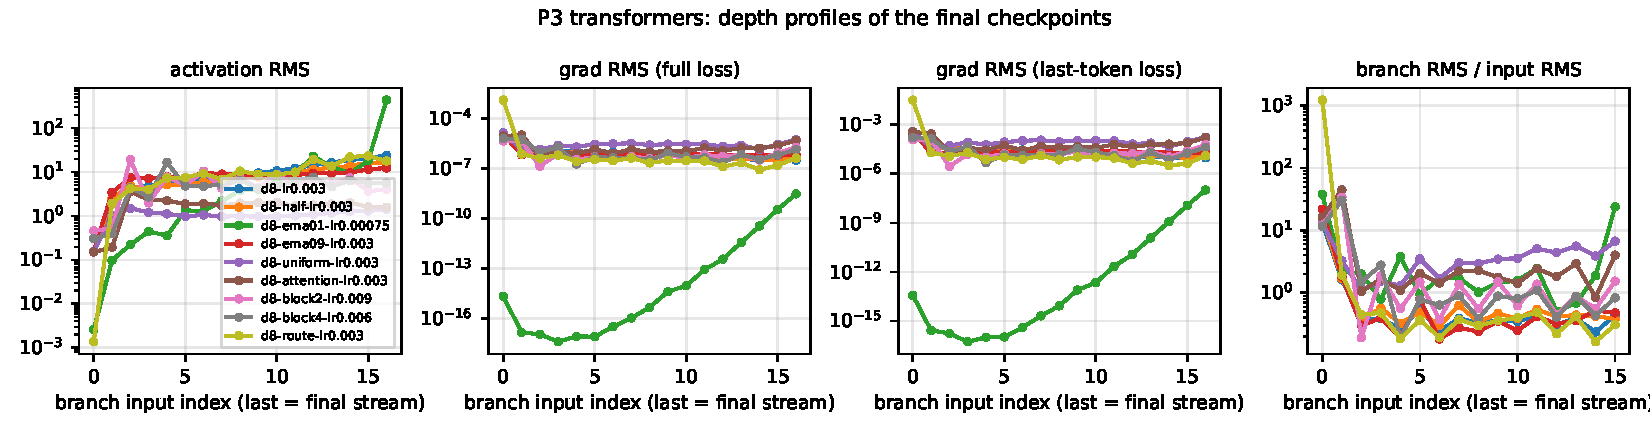
\includegraphics[width=\linewidth]{p3_t_depth_final.pdf}
\caption{P3 transformers: final checkpoints at each variant's best rate.}
\label{fig:p3t}
\end{figure}
\begin{figure}[h]\centering
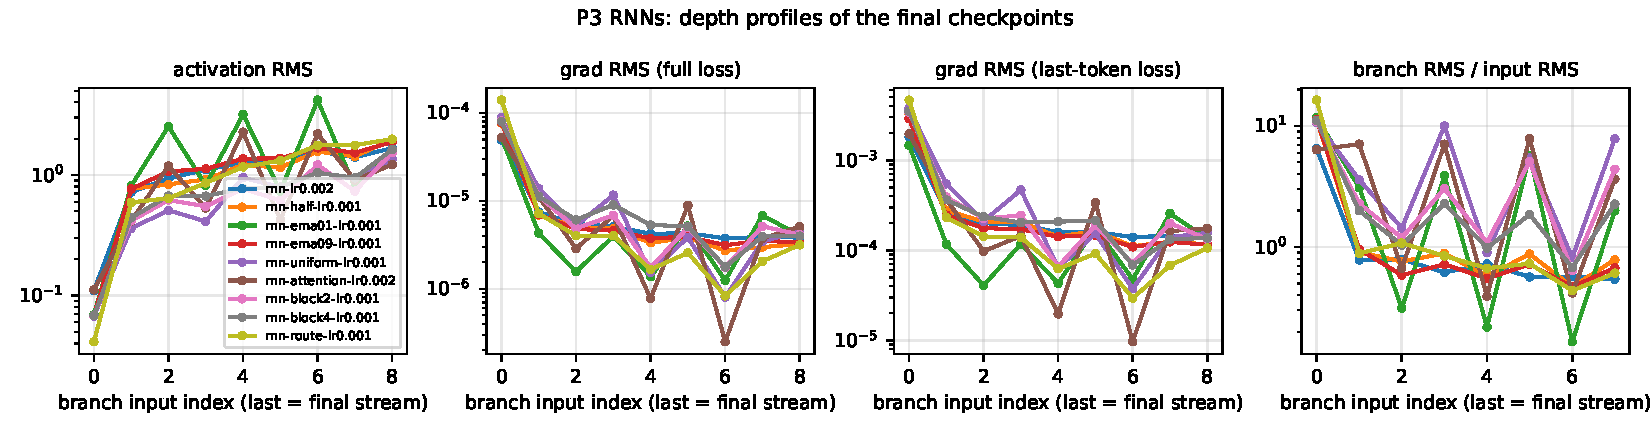
\includegraphics[width=\linewidth]{p3_r_depth_final.pdf}
\caption{P3 modern RNNs: final checkpoints at each variant's best rate.}
\label{fig:p3r}
\end{figure}
\begin{figure}[h]\centering
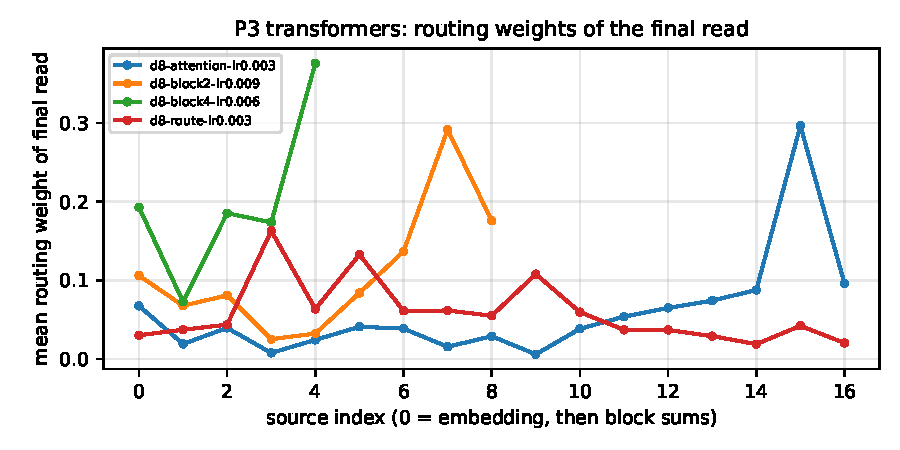
\includegraphics[width=.6\linewidth]{p3_t_routing.pdf}
\caption{Mean routing weights of the final read for the routed transformers.}
\label{fig:p3route}
\end{figure}


\section{P4: Recurrent updates}
\paragraph{Ablations.} Three GRU ablations isolate the parts of the gated update, each run at the GRU centre rate $\lr=0.003$ because each GRU style run costs about 90 minutes on an H100:
\begin{itemize}\setlength\itemsep{0pt}
  \item \texttt{gru-noreset}: $r\equiv 1$, the candidate always reads the whole hidden state.
  \item \texttt{gru-inputgate}: $r$ and $z$ are computed from $x_t$ only (no recurrent term in the gates); the candidate still reads $r\odot h$.
  \item \texttt{gru-linear}: the candidate drops its tanh, so the update is a gated linear map of $(x_t, r\odot h)$.
\end{itemize}

\paragraph{New update: decoupled forget and write gates.} The GRU writes with a convex combination $h' = (1-z)h + z\tilde h$, so it cannot keep $h$ and add new content at the same time, and it cannot clear $h$ without writing the candidate at full strength. My cell separates the two decisions and drops the reset gate:
\[
f_t = \sigma(W_f x_t + U_f h_{t-1}),\quad i_t = \sigma(W_i x_t + U_i h_{t-1}),\quad \tilde h_t = \tanh(W x_t + U h_{t-1}),\quad h_t = \phi\!\left(f_t\odot h_{t-1} + i_t\odot \tilde h_t\right),
\]
with the same parameter count as the GRU (three input and three recurrent matrices). Only $h$ is carried across time. \texttt{gru-dual} uses $\phi = \mathrm{id}$; \texttt{gru-dualnorm} uses a parameter free RMS normalisation $\phi(v) = v/\mathrm{rms}(v)$, which keeps the hidden state on the unit RMS sphere so that the unbounded $f\odot h + i\odot\tilde h$ sum cannot grow or shrink across 1024 steps. Classes \texttt{DualGateCell} and \texttt{DualGateNormCell} in \texttt{p4\_recurrent\_updates.py}.

\subsection{Runs and losses}
Table~\ref{tab:p4} lists the P4 runs. The GRU was swept over four rates because its best rate kept moving up: 3.231 at 0.0015, 3.188 at 0.003, 3.183 at 0.006 and 3.457 at 0.012. At its best it is 0.33 nats better than the supplied tanh modern RNN (3.516) with the same depth stack and 2.5 times its recurrent parameters, and it closes 55\% of the gap to the d8 transformer (2.927). My dual gate cell with RMS normalisation reaches 3.387 at 0.003 (3.605 at 0.006): better than every tanh RNN in P2 and P3 but 0.2 behind the GRU. Without the normalisation the same cell produced non-finite losses at step 1866 ($\lr=0.003$) and step 827 ($\lr=0.0015$), and I stopped both runs; the unnormalised sum $f\odot h + i\odot\tilde h$ can grow by up to one unit of RMS per step, and once the hidden state is large the tanh candidate and the gates saturate and the bf16 forward overflows.
\ablationparagraph

\begin{table}[h]\centering\small
\caption{P4 runs. Losses are FP32 recomputations on the saved checkpoints.}
\label{tab:p4}
\begin{tabular}{lp{0.78\linewidth}}\toprule
variant & final validation loss per peak rate\\\midrule
rnn, tanh cell (supplied) & $\lr$=0.002: 3.516 (best of five) \\
gru & $\lr$=0.0015: 3.230; $\lr$=0.003: 3.188; $\lr$=0.006: \textbf{3.183}; $\lr$=0.012: 3.457 \\
gru-noreset & $\lr$=0.003: \textbf{3.285} \\
gru-inputgate & $\lr$=0.003: \textbf{3.235} \\
gru-linear & $\lr$=0.003: diverged (NaN) \\
gru-dual & $\lr$=0.0015: diverged (NaN); $\lr$=0.003: diverged \\
gru-dualnorm & $\lr$=0.003: \textbf{3.387}; $\lr$=0.006: 3.605 \\
\bottomrule\end{tabular}

\end{table}

\subsection{Checkpoint behaviour against the tanh baseline}
Figure~\ref{fig:p4time} shows why the GRU wins. Its last layer hidden state has RMS 0.4 instead of 0.9 and fewer than 1\% of its units are saturated against 50\% for the tanh cell, so the convex update $h' = (1-z)h + z\tilde h$ keeps the state in the linear range of the nonlinearity. Under the last token loss its hidden state gradient is flat at $10^{-7}$ to $10^{-6}$ across all 1024 steps, where the tanh cell's gradient underflows after 90 steps: the $(1-z)$ path is an identity through time whenever the update gate is closed. The full loss gradient is 10 to 30 times larger than the tanh cell's at every step. The context tests (Table~\ref{tab:p4ctx}) agree: dropping context beyond 64 tokens still costs the GRU 0.13 nats and beyond 256 tokens 0.01, where the tanh RNN gains nothing beyond 64 tokens, and the GRU does not depend on the first token (2.6 nats with one token of context whether or not the first token is restored, against 42 nats for the tanh RNN without it). Its upper layers hold a smooth state (cosine 0.84 between $h_t$ and $h_{t-64}$ in layer 4) without freezing.

The dual gate cell with normalisation shows the failure mode of its design: the hidden state cosine at lag 64 is 0.99 to 1.00 in layers 2 to 4, that is, the normalised state converges to a fixed direction and the upper recurrent layers stop carrying information in time; the model then behaves like a one layer recurrence plus feedforward blocks, which is what its loss (3.387) says. It also inherits the first token dependence of the tanh model (263 nats with one token and no first token). Normalising $h$ removed the overflow but also removed the scale the gates need to express forgetting.

\begin{figure}[h]\centering
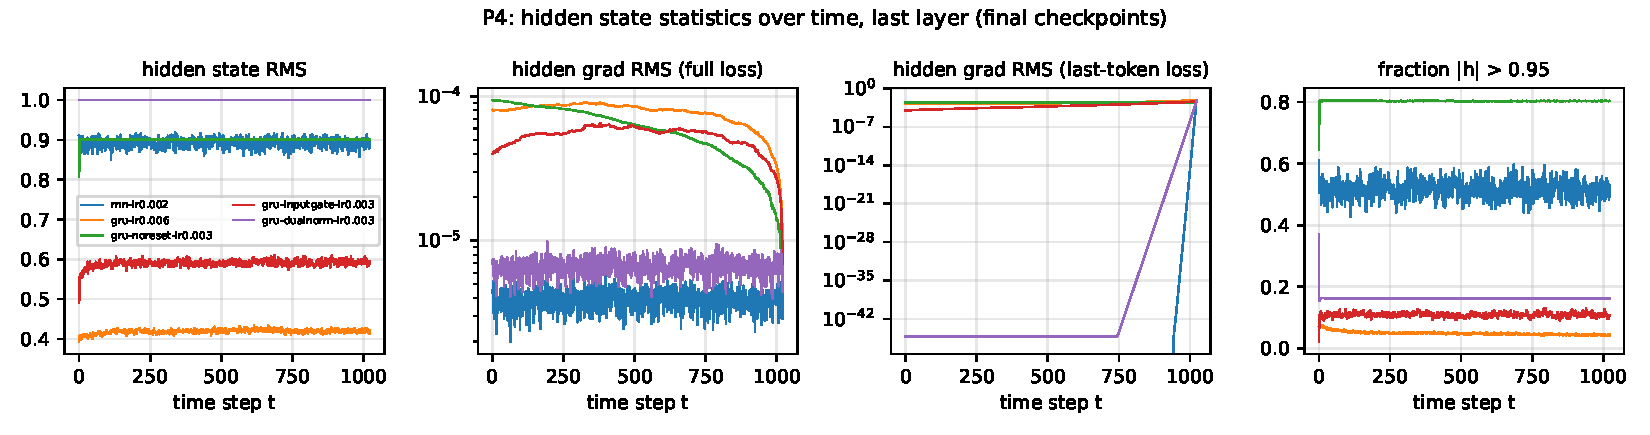
\includegraphics[width=\linewidth]{p4_temporal.pdf}
\caption{P4: last recurrent layer over time for the tanh modern RNN, the GRU and the dual gate cells (final checkpoints).}
\label{fig:p4time}
\end{figure}

\begin{table}[h]\centering\small
\caption{P4 context tests: increase of the last token loss (nats) with $k$ recent tokens; final checkpoints.}
\label{tab:p4ctx}
\begin{tabular}{llrrrrr}\toprule
model & first token & $k=1$ & 4 & 16 & 64 & 256\\\midrule
tanh modern RNN & dropped & 42.3 & 54.9 & 56.1 & 49.1 & 39.3\\
tanh modern RNN & restored & 1.91 & 0.50 & 0.16 & 0.00 & 0.00\\
GRU ($\lr$=0.006) & dropped & 2.57 & 0.85 & 0.28 & 0.13 & 0.01\\
GRU ($\lr$=0.006) & restored & 2.11 & 0.75 & 0.17 & 0.11 & 0.01\\
dual gate, normalised & dropped & 263 & 82.3 & 4.94 & 0.59 & 6.52\\
dual gate, normalised & restored & 1.95 & 0.48 & 0.08 & 0.04 & 0.00\\
\bottomrule\end{tabular}
\end{table}


\section{A competitive RNN against the transformer}
The best RNN of the whole study is compared with the baseline transformer here on the same probes (the P4 section reports which RNN that is; this section uses the supplied modern tanh RNN at $\lr=0.002$ and the d8 baseline at $0.003$ because both have every probe, and the P4 figures show the same statistics for the GRU family). Figure~\ref{fig:cmp} plots the activation RMS of the residual stream at every position and the cosine between stream states at different positions, per depth index.

\paragraph{Across layers.} Both models grow their stream with depth and change its direction mostly in the first two branches (Figures~\ref{fig:p1stages} and~\ref{fig:p2stages}), but the scales are very different: the transformer stream ends at RMS 24 and the RNN stream at 1.7, because the RNN's recurrent branches pass through a tanh and its MLP outputs stay near the stream scale, while the transformer's first attention and MLP branches emit outputs 6 to 20 times their input. The transformer's full loss gradient decays by 50 from embedding to final stream and the RNN's by 10, so the RNN's depth is, if anything, better conditioned; its problem is time, not depth.

\paragraph{Across positions.} The transformer has one special position. At $t=0$ its final stream RMS is 90, four times the 22 to 25 at every other position, which is the massive activation that every head attends to as a sink (Section 2.3). The RNN has the opposite special position: its state at $t=0$ is small (RMS 0.5 against 1.6 to 1.8 later) because the recurrence starts from zero and needs a few steps to reach its working range. Away from $t=0$ the RMS of both models is flat in position. The cosine between stream states one position apart rises from 0.05 at the embedding to 0.45 to 0.5 in the transformer's middle and upper layers and stays near that value for lag 64 and for the cosine to the first position (0.25 to 0.35): the transformer keeps a shared, position independent component (the sink direction and a mean token direction) plus a token specific part. The RNN's lower layers have almost orthogonal states at adjacent positions (cosine 0.1 for layers 1 and 2) and its upper layers reach 0.48, similar to the transformer, but their similarity falls off faster with lag (0.36 at lag 64, 0.34 to the first position). Measured on the hidden states themselves rather than the stream, the RNN's upper layers are far smoother in time (cosine 0.93 at lag 64 in layer 4, Section 3.2), so the recurrent branches carry a slow state and the stream adds a fast, token specific component through the MLPs. The gated residual variants of both families have lower cross position similarity at every depth (transformer 0.2 to 0.3 at lag 64, RNN 0.02 to 0.15), that is, the gates remove some of the shared component.

\paragraph{Context.} The practical difference is in Table~\ref{tab:p2ctx} and Figure~\ref{fig:p1ctx}: the transformer still improves from tokens 256 to 1023 and loses 1.7 nats when cut to 16 tokens, whereas the RNN gains nothing measurable beyond 64 tokens and its last token gradient underflows within 90 steps. The transformer's 0.4 nat advantage in full loss (2.83 against 3.33 on the probe sequences) is the long context it can use and the RNN cannot.

\begin{figure}[h]\centering
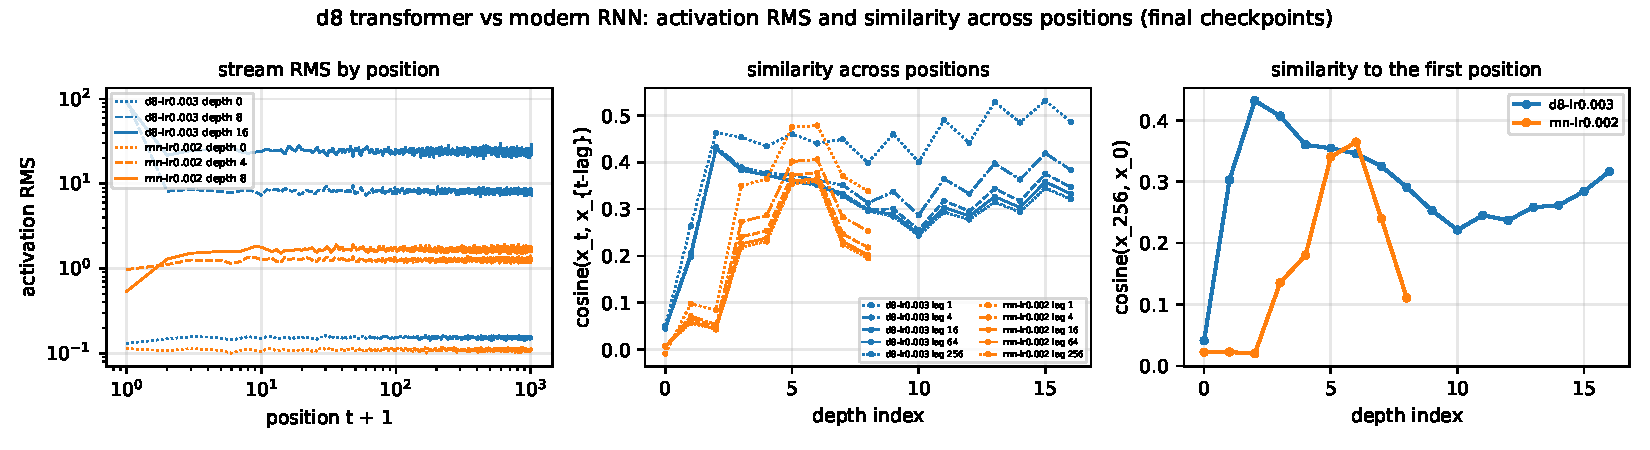
\includegraphics[width=\linewidth]{cmp_positions.pdf}
\caption{Transformer d8 against the modern RNN. Left: stream RMS at every position for the embedding, the middle branch input and the final stream. Middle: cosine between stream states at lags 1 to 256 against depth. Right: cosine between position 256 and position 0.}
\label{fig:cmp}
\end{figure}

\section{Divergent and failed runs}
\begin{itemize}\setlength\itemsep{0pt}
\item Non-finite gradients (run stopped by the clipping check): d8-no-prenorm at $\lr=0.002$ (step 747) and $0.004$ (step 82); rnn-no-prenorm at $0.004$.
\item Collapsed to the unigram loss 6.875 without a NaN: d8-no-residual at all five rates; d8-postnorm at $0.004$; rnn4 at $0.002$ and $0.004$.
\item Trained but far off the sweep: d8-no-qknorm at $0.006$ (3.83) and $0.012$ (4.20); rnn-postnorm at $0.002$ (4.26) and $0.004$ (6.39), whose global activation RMS peaked near 4000 before it fell back.
\item Probe failures: the final checkpoint of rnn-gated-norm at $\lr=0.001$ was not probed in the first CPU batch and was rerun with the P3/P4 probes.
\studentfailures
\end{itemize}

\appendix
\section{Additional depth profiles}
\begin{figure}[h]\centering
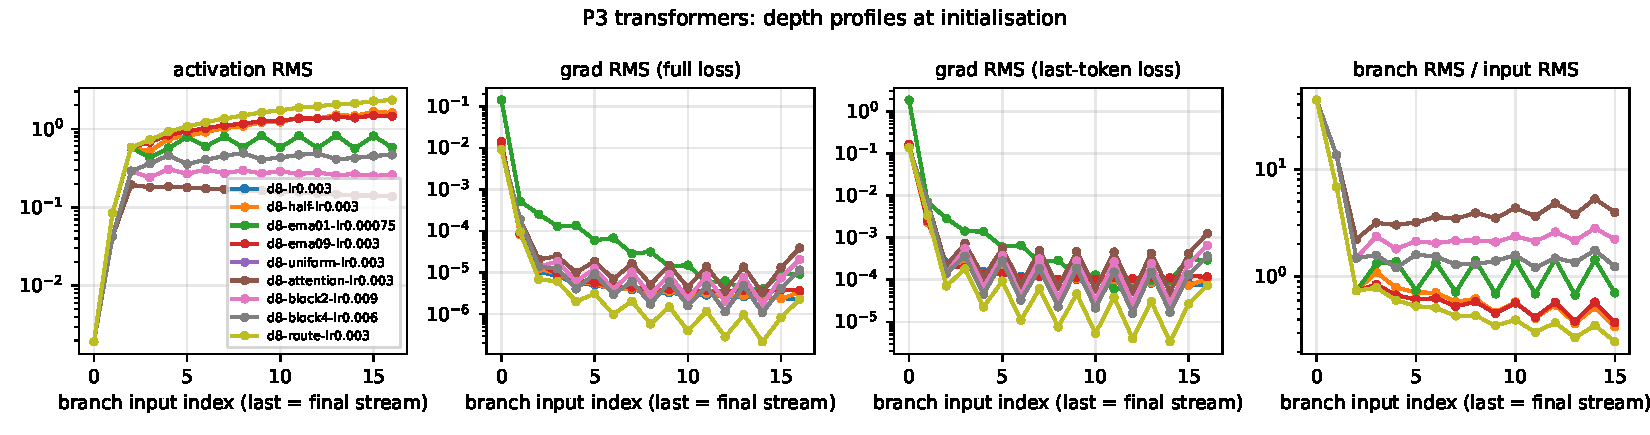
\includegraphics[width=\linewidth]{p3_t_depth_init.pdf}
\caption{P3 transformers at initialisation (seed 42). The gated route model is identical to the baseline here.}
\label{fig:p3ti}
\end{figure}
\begin{figure}[h]\centering
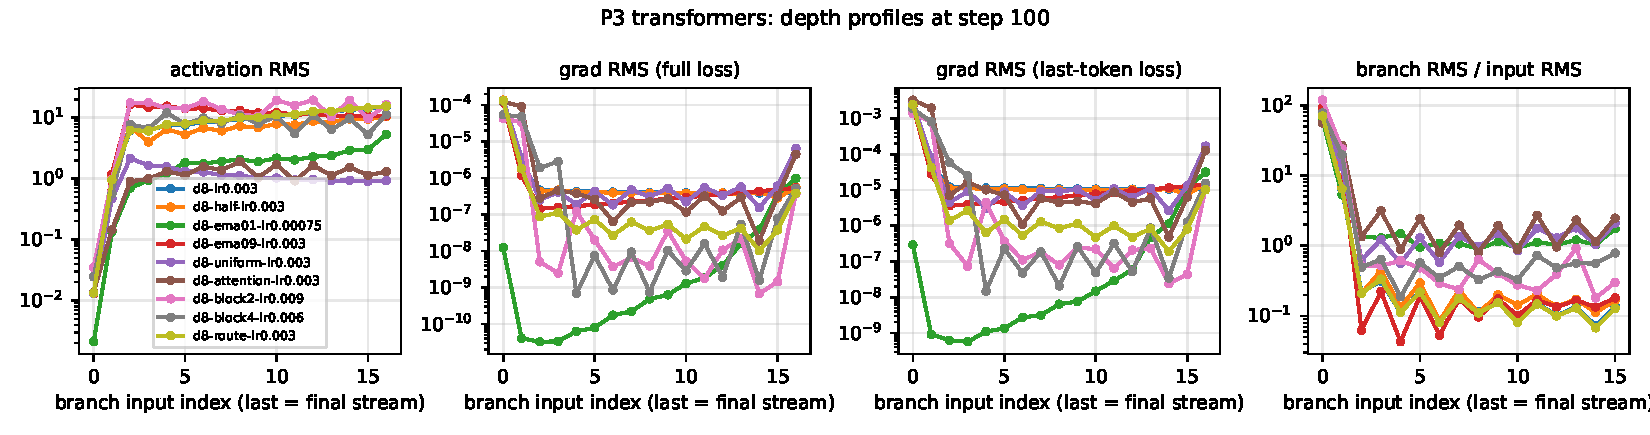
\includegraphics[width=\linewidth]{p3_t_depth_early.pdf}
\caption{P3 transformers at step 100.}
\label{fig:p3te}
\end{figure}
\begin{figure}[h]\centering
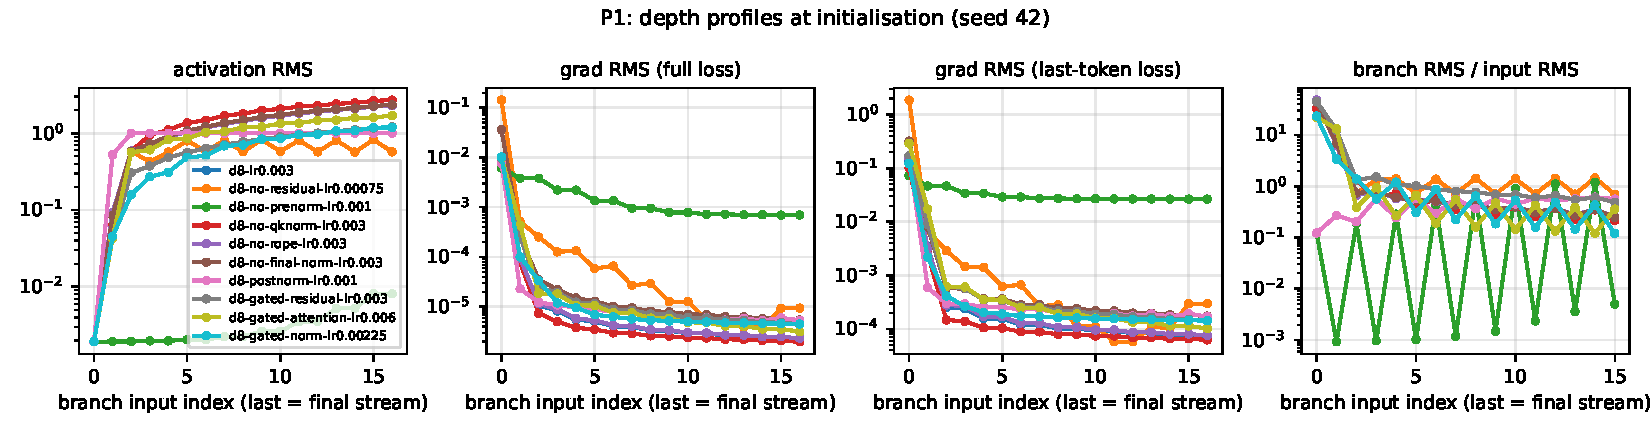
\includegraphics[width=\linewidth]{p1_depth_init.pdf}
\caption{P1 transformers at initialisation.}
\label{fig:p1init}
\end{figure}


\end{document}
